\chapter{Analysis using Formalized Claims}
\label{chap:analysis}


Throughout the thesis, we advocate for formalized over unstructured claims,
since a subsequent argumentation analysis different kind of information.  In a
formalized setup, we may derive implicit claims with exact inference, compared
to the unstructured setup (as laid out in chapter~\ref{chap:deriving_implicit})
where information retrieval proves to be much less informative.  Formalized
claims can be easily queried and are not ambiguous as unstructured claims might
be. 

% TODO transfer to introduction
% Not being able to determine why a causal relationship exists between two claims
% 
% is one of the main criticisms of machine learning 
% \citep{pearl1998graphs}

% The biggest disadvantage of using formalized claims is losing the free-form 
% expressiveness which unstructured claims provide. 

In this chapter, we scratch the surface of argumentation analysis by
demonstrating the applications of formalized claims.  More specifically, we
demostrate the benefits of formalized claims by analyzing the ``\emph{Gay
Rights}'' and the ``\emph{Marijuana}'' topics. 
We use microstructures to do stance classification in
section~\ref{sec:stance_micro}, analyze most frequently used
claims, and provide guidelines for other types
of analysis in section~\ref{sec:implicit_formalization}. 

% Finally, we provide 
% conclusions and guidelines for other types of analysis that could be 
% conducted with formalized claims in section~\ref{sec:struc_conclusion}. 

\section{Stance Classification using Microstructures}
\label{sec:stance_micro}

\begin{table}[t]
\begin{center}
{%\footnotesize
\begin{tabular}{p{0.75\columnwidth}c c}
\toprule
& \multicolumn{2}{c}{\textbf{Stance}}\\
\cmidrule(lr){2-3}
\textbf{\textbf{Claim paraphrase}} & \textbf{A1} & \textbf{A2} \\
\midrule
\emph{Gay couples should be able to experience parenting.} & F & F \\
\midrule
\emph{Gay couples don't have children.} & N & N \\
\midrule
\emph{By natural means, infertility is wrong.} & a & a \\
\midrule
\emph{A homosexual relationship lacks the ability to procreate.} & a & A  \\
\bottomrule
\end{tabular}}
\caption{Claim paraphrase 
	stance annotations towards the topic of ``\emph{Gay Rights}''.}
\label{tab:microstructure_stance}
\end{center}
\end{table}

We show how microstructures (defined in section~\ref{sec:for_microstructures})
can be used for stance classification. 

\paragraph{Data.} We use a subset  of the ``\emph{Gay Rights}'' dataset defined in
section~\ref{sec:claim_seg_data} for which annotators could produce 
a microstructure (819 out of 920 claims). We then ask two annotators to label
stance for each of the 819 claim paraphrases on a five-point scale:
\emph{strong favor} (\textbf{F}), \emph{likely favor}(\textbf{f}), \emph{neither} (\textbf{N}),
\emph{likely against} (a), and \emph{strong against} (\textbf{A}). 
We adopt the definition of \textbf{F}, \textbf{N}, and \textbf{A} stance from 
\citep{mohammad2016semeval}, with the addition of the in-between options
(\textbf{f} and \textbf{a}) for indicating implicit or indirect stance. 
Table~\ref{tab:microstructure_stance} shows example stance-annotated  
claim paraphrases. On the five classes, we observe a moderate inter-annotator
agreement of 0.53 Cohen's $\kappa$ \citep{cohen1960coefficient}.
The aggregation of labels was done by removing 16 instances on which the
annotators disagreed in stance polarity, then averaging and rounding two labels
by treating them as numbers from the $[-2, \mathop{+}2]$ interval.
Finally, we end up with 803 claim (segmented from comments) with an 
associated claim paraphrase, microstructure, and stance. 

\paragraph{Baselines.} 
We compare against two baselines, which, to the best of our knowledge, are
considered state of the art methods for stance classification
\citep{sobhani2016detecting}: 
\begin{enumerate*}[label=(\arabic*)]
\item a sum of skip-gram vectors \citep{mikolov2013distributed} for each word
and a
\item tf-idf unigram and bigram representation of a claim.
\end{enumerate*}
For baselines, we use these representations of original claim segments
(\emph{seg}). For the sake of completeness, we also run 
the baselines on claim paraphrases (\emph{par}), but note that this serves
only as a reference, as obtaining paraphrases is arguably a task 
that is more difficult than obtaining microstructures. 

\paragraph{Microstructures.}
To represent the claim microstructures (\emph{ms}), we adopt a simple 
one-hot vector for each microstructure component: modality, relations, 
relation negations, concepts, and opinion holders.
Then we concatenate the vectors into a single feature vector (\emph{onehot}). 
In addition, to leverage the taxnomical relations between concepts, 
we experimented with encoding for each concept its ancestors in the taxonomy
by encoding the nodes along the path leading from the root to the concept (\emph{path}).

\paragraph{Models. }
We used support vector machine (SVM) classifier and regression models with an
RBF kernel, as implemented in the LibSVM library of \citet{chang2011libsvm}.
We trained and evaluated the models on 803 claim instances
(either original segments, paraphrases, or microstructures) using
$5 \times 3$ nested cross validation, using grid-search to 
optimize hyperparameters $C$ and $\gamma$
(model selection explained in section~\ref{sec:selection}).

\paragraph{Tasks.}
We considered four tasks:
\begin{enumerate*}[label=(\arabic*)]
\item a 5-way regression, in which the model is trained to predict the
numeric stance score, but afterwards predictions are rounded and mapped to labels,
\item a 5-way classification task,
\item a 3-way classification task, in which the implicit labels (\textbf{a} and \textbf{f}) are
mapped to neutral (3-way-N), and
\item a 3-way classification task, in which the implicit labels are mapped to
explicit \pro{for} and \con{against} labels (3-way-E)
\end{enumerate*}
Since the solution space is more narrow for the last two tasks, 
we expect models to perform these tasks better. 


\begin{table}[t]
\begin{center}
{
\setlength{\tabcolsep}{5pt}
\begin{tabular}{l cccc}
\toprule
& \textbf{Regression} & \multicolumn{3}{c}{\textbf{Classification}}\\
\cmidrule(lr){2-2}\cmidrule(lr){3-5}
\textbf{Features} & \textbf{5-way} & \textbf{5-way} & \textbf{3-way-N} & \textbf{3-way-E} \\
\midrule
%\emph{majority}  &           0.069  &     	0.082 &             0.091                    & 	0.205 \\
\emph{seg-w2v}    &      0.084  &      \textbf{0.230} &             \textbf{0.259}                     &   \textbf{0.383} \\
\emph{seg-tfidf}      &      \textbf{0.133}  &      0.170 &             0.248                     &   0.297 \\
\midrule
\emph{par-w2c}   &       0.133  &      0.170 &             0.248                     &   0.297 \\
\emph{par-tfidf} &       \textbf{0.250}  &      \textbf{0.290} &             \textbf{0.487}                     &   \textbf{0.377} \\
\midrule
\emph{ms-onehot} &       0.316  &     	\textbf{0.320} & 	\textbf{0.507}                    &   \textbf{0.473} \\
\emph{ms-path}  &  \textbf{0.331}  &     	0.315 &         	0.501                    &    0.462 \\
\bottomrule
\end{tabular}}
\caption{Claim stance classification macro-averaged F1-score using segments
	(\emph{seg}), paraphrases (\emph{par}), and microstructures \emph{(ms)}
	as features. The best result in each group is shown in boldface.}
\label{tab:microstructure_stance_experiment}
\end{center}
\end{table}

\paragraph{Results. }
Table~\ref{tab:microstructure_stance_experiment} shows the classification
results in terms of macro-averaged F1-score.  As expected, the 3-way
classification tasks are easier to solve than the 5-way classification tasks.
Furthermore, the 5-way regression model performs better the 5-way classifier,
suggesting that using distance-sensetive loss is beneficial for this
task. In all four tasks, claim microstructures considerably outperform
both segment-based baselines, yielding between 9 and 25 points of
improvement in F1-score, depending on the task.
All differences between the baseline and the microstructure model 
are statistically significant at $p < 0.05$ (tested using
a two-tailed permutation test as described by \citet{yeh2000more}).
By comparing with claim paraphrases, we find that microstructures give
comparable performance for 5-way and 3-way-N classification tasks
(the differences are not statistically significant at $p < 0.05$),
while for 5-way regression and 3-way-E classification tasks
the microstructures outperform paraphrase representations. Finally, 
the performance difference between one-hot encoded microstructures
and microstructures with path-encoded concepts are not statistically
significant at $p < 0.05$, suggesting that stance classification did not
profit from encoding taxonomical relations. 
Microstructures improve claim stance classification performance over 
segment-based baseline by a maximum of 50.7\% macro-averaged F1-score
for a 3-way classification setup.

\section{Implicit Claims using Formalizations}
\label{sec:implicit_formalization}

We wish to explore discovering implicit claims in a structured manner. 
An unstructured approach to discovering implicit claims 
was presented in chapter~\ref{chap:deriving_implicit}. There it was clearly
shown how using implicit claims improves the task of prominent 
claim identification, but it proved extremely difficult to automatically retrieve 
implicit claims (shown in section~\ref{sec:argpremise_retrieval}). 
Now, we show an analysis of formalized claims which uses inference to uncover
implicit claims to demonstrate one of the advantages of structured
argumentation mining. 

We propose four tasks in the analysis. For the first three tasks, 
we demonstrate how implicit claims can impact frequency counts.
We search for the most frequently used claims using different sets
of claims. More specifically, in the first task we count 
the frequencies of asserted claims. In the second task, we 
calculate frequencies for both asserted and inferred
claims. For the third task, we add custom axioms which produce implicit claims,
which we then add with the asserted and inferred claims, before
doing another frequency count. In the fourth task, we analyze claims
across different speakers and propose \emph{crowd-based} inference.

We use the \emph{ClaimOntology} and the \emph{marijuana legalization} domain
presented in chapter~\ref{chap:formalization}. Most frequent queries 
are made using Java libraries OntoAPI \citep{bellatreche2007ontoapi} and 
the JFact reasoner\footnote{\url{http://jfact.sourceforge.net/}}.
Queries to filter claims are made using the SPARQL query language
\citep{perez2006semantics}.

\subsection{Task \rom{1}: Asserted Implicit Claims}

\begin{table*}[t]
\centering
\begin{tabular}{p{9 cm} | cc | cc | cc}
	\toprule
	\textbf{Claim} & freq & rank & freq & rank & $\Delta$rank \\
\midrule
	\emph{Marijuana should be legal 				}& 35 & 1 & 39 & 1 & 0 \\
	\emph{Marijuana should be illegal 				}& 22 & 2 & 22 & 3 & -1 \\
	\emph{Marijuana consumption causes reduced mental capabilities} & 10 & 3 & 18 & 2 & +1 \\
	\emph{Marijuana promotes mind influental behavior 		}& 10 & 3 & 17 & 5 & -2 \\
	\emph{Marijuana consumption promotes negative health effects 	}& 10 & 3 & 23 & 2 & +1 \\
\bottomrule 
\end{tabular}
\caption{Claim frequency in the domain independent setup. Frequency and rank are
	shown before and after adding inferred claims. }
\label{tab:claim_freq_indep}
\end{table*}

We wish to explore most frequently used claims in two ways.
First, we determine the most frequent claims across the entire dataset
(\emph{domain independent}).
Second, most frequently used claims across a specific 
(``\emph{marijuana legalization}'') domain filter query
(\emph{domain dependent}). 
Two claims individuals are equivalent if they both contain the same
object properties, data properties, and domain individuals. 

In the domain independent setup, we use 864 formalized claims (56 are excluded
from the total dataset of 920 claims since they were not deemed
suitable for formalization). Out of 864 claims there are 477 unique claims. 
The mid column of table~\ref{tab:claim_freq_indep} shows most frequent claims.
The top two claims express \pro{pro} (rank \#1) and \con{con} (rank \#2) stance 
towards the topic. The next top claims outline reasons behind the one of these 
stances. 

For the domain dependent setup, we filter out part of the dataset. We make a
SPARQL query that targets claim individuals which contain the \texttt{causes} property
and the \texttt{marijuana} domain individual: 
{
\small{
\begin{verbatim}
PREFIX rdf: <http://www.w3.org/1999/02/22-rdf-syntax-ns#>
PREFIX owl: <http://www.w3.org/2002/07/owl#>
PREFIX rdfs: <http://www.w3.org/2000/01/rdf-schema#>
PREFIX xsd: <http://www.w3.org/2001/XMLSchema#>
PREFIX leg_mar:
<http://www.semanticweb.org/ontologies/2018/2/legalized_marijuana#>

SELECT ?subject ?object
	WHERE { ?subject leg_mar:has_antecedent leg_mar:marijuana .
                ?subject leg_mar:causes ?object}
\end{verbatim}
}
}

After filtering, we again determine the most frequent claims (shown in 
table~\ref{tab:claim_freq_dep}). We observe that speakers usually talk 
about different negative health effects marijuana causes, such as 
memory damage or motoric diseases. However, we can notice that 
some claims infer others: \emph{marijuana causes some disease} infers
all claims that mention some specific disease (such as 
\emph{marijuana causes motoric disease}. 

\begin{table*}[t]
\centering
\begin{tabular}{p{9 cm} | cc | cc | cc | c}
	\toprule
	\textbf{Claim} & freq & rank & freq & rank & $\Delta$rank \\
\midrule
	\emph{Marijuana causes negative health effects                  }& 10 & 1 & 10 & 1 & 0\\
	\emph{Marijuana causes brain memory damage                      }& 4 & 2 & 4 & 4 & +2\\
	\emph{Marijuana causes motoric disease                          }& 4 & 2 & 4 & 4 & +2\\
	\emph{Marijuana causes positive mind influence                  }& 3 & 4 & 3 & 6 & +2 \\
	\emph{Science believes marijuana causes negative health effects }& 2 & 5 & 2 & 9 & +4 \\
	\emph{Marijuana causes death                                    }& 1 & 10 & 5 & 3 & -7 \\
	\emph{Marijuana causes some disease                             }& 0 & N/A & 10 & \textbf{1} & N/A \\
\bottomrule 
\end{tabular}
\caption{Claim frequency in domain dependent setup. Frequency and rank are
	shown before and after adding inferred claims.  }
\label{tab:claim_freq_dep}
\end{table*}

\subsection{Task \rom{2}: Ontology-Inferred Implicit Claims}

Implicit claims can be inferred from asserted claims by taking advantage
of the superproperties and superclasses in the ontology. 
For example, we can derive an inferred claim
\emph{marijuana promotes motoric disease} from the claim 
\emph{marijuana causes motoric disease}
since the \texttt{promotes} object property is a superproperty of the
\texttt{causes} object property. 
Looking at the domain ontology, \texttt{some disease} is defined an individual 
of the \texttt{disease} class, whereas \texttt{motoric disease} belongs to a 
subclass of the \texttt{disease} class.
Therefore, the claim individual \emph{marijuana causes motoric disease}
infers the implicit claim individual \emph{marijuana causes some disease}. 
We now add inferred claims based on superproperties and 
superclasses to the entire dataset. 

The results of frequency counting for the domain independent setup 
are listed in columns 3 and 4 of table~\ref{tab:claim_freq_indep}. 
Comparing the frequencies after inference to the ones before, we can observe
that the claim \emph{marijuana consumption promotes negative health effects}
becomes a much more prominent claim by rising from 10 occurences to 23.

\subsection{Task \rom{3}: Axiom-Inferred Implicit Claims}

Inferring through axioms from the domain or upper ontology is useful, 
but some argumentation expert might want to interact with the ontology to
uncover additional implicit claims. Such an expert may then 
add his knowledge via axioms. Some axioms can be domain 
indepedent, such as the transitivity of the \texttt{causes} object property.
Other axioms may be domain dependent like stating
that a positive value statement about the \texttt{marijuana} domain 
individual inferrs an implicit claim individual that contains
 a \texttt{policy} modality and \texttt{has\_declaration} 
 object property with \texttt{marijuana legalization} domain individual.

Transitivity is defined as $\forall a, b, c \in X : (a R b \vee b R c)
\Rightarrow a R c$, where $X$ is the domain of concepts and $R$ is the
\texttt{causes} binary property between concepts. Defined in terms of the ontology, 
we derive a transitive implicit claim (3) if 
there exists a speaker who made two claims with properties like (1) and (2):
\begin{align*}
	(1) & \hspace{0.1cm} \mathit{has\_antecedent} (a)  \wedge  \mathit{causes} (b) \\
	(2) & \hspace{0.1cm} \mathit{has\_antecedent} (b) \wedge \mathit{causes} (c) \\
	\cline{1-3}
	(3) & \hspace{0.1cm} \mathit{has\_antecdent} (a) \wedge \mathit{causes} (c)
\end{align*}
where $a, b, c$ are domain individuals. For example, if we take two claims
stating
\emph{marijuana legalization causes marijuana taxation} and 
\emph{marijuana taxation causes economy profit}, the derived transitive
implicit claim amounts to \emph{marijuana legalization causes economy profit}.
We apply this rule for \texttt{causes}, \texttt{promotes}, and \texttt{implies}
object properties which yields 26 inferred claims. 

As for domain dependent axioms, an expert may want to encode that 
speakers who express positive value judgements about 
\texttt{marijuana legalization} also \pro{support} it by making 
a policy statement. 
Now, we define a policy implicit claim with properties (2)  if there
exists a claim with properties (1):
\begin{align*}
	(1) & \hspace{0.1cm} \mathit{has\_declaration} (\mathit{marijuana}) 
	\wedge \mathit{has\_modality} (\mathit{good\_value})\\
	\cline{1-3}
	(2) & \hspace{0.1cm} \mathit{has\_declaration} (\mathit{marijuana}) 
	 \wedge \mathit{has\_modality} (\mathit{policy})
\end{align*}
We apply this rule using the \texttt{marijuana}, \texttt{marijuana
legalization}, and \texttt{marijuana consumption} domain individuals.
Additionally, we apply the equivalent rule, with the difference of requiring
the \texttt{bad\_value} modality, to derive claims which are \con{against}
\texttt{marijuana legalization}. Applying these rules to the dataset increases
the frequencies of claims \emph{marijuana should be legalized} and {marijuana
shouldn't be legalized} from 35 to 39 and 22 to 37 respectively.  This
indicates that negative stance is implicit much more often than positive
stance. 

\subsection{Task \rom{4}: Collective-Inferred Claims}

\begin{table*}[t]
	\tiny{
		\begin{tabular}{p{1cm} | p{1.6cm} p{1.65cm} p{1.65cm} p{1.65cm} |  p{1.65cm} p{1.65cm} p{1.65cm} p{1.65cm}}
	\toprule
			\multirow{2}{*}{\parbox{1cm}{Concomitant \\ Claims}} &

	\multicolumn{4}{c|}{\pro{Marijuana should be legalized}}
	& \multicolumn{4}{c}{\con{Marijuana should not be legalized}} \\[1ex]

	& 
	\multicolumn{4}{c|}{\pro{Marijuana should be taxed}} 
	& \multicolumn{4}{c}{\con{Marijuana has negative effects on the human body}} \\[2ex]

	% speakers
	Speaker & 
	\multicolumn{1}{c}{\small{E12}} &
	\multicolumn{1}{c}{\small{K1}}  &
	\multicolumn{1}{c}{\small{K97}} &
	\multicolumn{1}{c|}{\small{K75}} &
	\multicolumn{1}{c}{\small{B48}} &
	\multicolumn{1}{c}{\small{I89}} &
	\multicolumn{1}{c}{\small{B58}} &
	\multicolumn{1}{c}{\small{K200}} \\[1ex]

	\hline

	& 
	Marijuana should be regulated & 
	Marijuana would be cheaper if legalized & 
	Alcohol causes more casualties than marijuana & 
	Marijuana legalizationcould be the answer to the U.S. debt crisis. &
	Marijuana is a drug &
	Marijuana is a drug & 
	Marijuana abuse kills people & 
	Marijuana is a drug \\
	\hline

	& 
	We should stop wasting money on monitoring & 
	If marijuana was legal, it would not be risky to sell marijuana. &
	There is nothing wrong with consuming marijuana & 
	& 
	Marijuana makes you hungry & 
	Marijuana contains more toxic substances than tobacco &
	Marijuana abuse causes mental illness &
	Marijuana is terrible \\
	\bottomrule
\end{tabular}
}
	\caption{Four \pro{pro} (left) and four \con{con} (right) 
	marijuana legalization speakers share two concomitant claims (up),
	and make additional unshared claims (down)
	}
\label{tab:struc_group}
\end{table*}

So far, we have derived implicit claims at either the speaker level, or across
the entire set. Now, we wish to see if we can identify groups of speakers with
concomitant claims. We adopt a collaborative filtering approach
\citep{herlocker1999algorithmic} to detect speakers sharing claims.  We take
(asserted and inferred) claims  from all previous analysis (1451 unique claims)
and observe claims which are shared amongst at least two distinct speakers.
We end up with 379 claims shared by at least two, and 174 claims shared by at least three
speakers. 

\begin{figure}[t]
	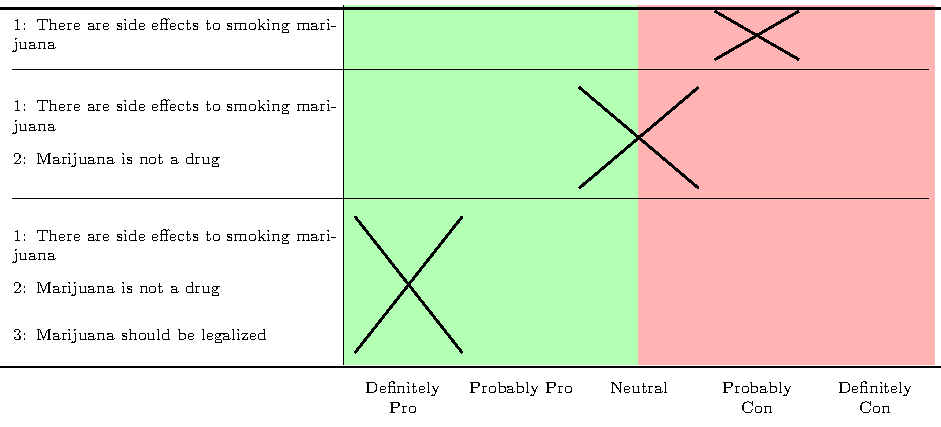
\includegraphics{struc_arg_shift-figure0.pdf}
\caption{Shifts pro con. The stance changes as more claims are uncovered. In the first row, 
a single claim is known, based on which the \con{con} stance is inferred.
As the second and third claim are uncovered the stance shifts towards neutral and 
\pro{pro} stance, respectively.
}
\label{fig:pro_con_shift}
\end{figure}


An example of concomitant claims is shown in table~\ref{tab:struc_group}. 
Two groups (one \pro{pro} and one \con{against} marijuana legalization)
of four speakers share exactly two claims. Looking at the \con{con} side, we
can infer that speaker $K200$ is also likely to claim that \emph{marijuana is a drug}, because
he shares claims with three other speakers that make that claim.
In the \pro{pro} group only speaker $K75$ makes a claim 
\emph{marijuana legalization will help the government earn money}, but
common sense reasoning and domain knowlege suggest that other speakers in the group
are likely to agree with that statement. Speaker $E12$ states 
that \emph{money is wasted on monitoring} and $K1$ states that \emph{
marijuana would be cheaper if legalized} which in real life situations 
would usually be associated with supporting the fact that it would
\emph{help the government earn more money}, but there is no direct line of inference.
The absence of such a claim suggests that more common-sense axioms could be
added to add extra implicit claims, but at the potential cost of 
implicit inferring something speakers might not have meant to be implied. 

To underline how easy it can be to imply incorrect claims, we show a series of
claims made by a speaker in Fig.~\ref{fig:pro_con_shift}.  The speaker first
makes the claim \emph{there are side effects to smoking marijuana}, which is a
claim that is often associated with the \con{con} stance, leading us to believe
the speaker is also \con{against} marijuana legalization.  However, after
making the claim \emph{marijuana is not a drug} the speaker is closer to the
claims more often expressed by supporters of marijuana legalization.  Finally,
the speaker expresses their \pro{pro} stance with the claim \emph{marijuana
should be legalized} removing any doubt. Having more claims usually leads to
better understanding of the speakers' opinion. 

Note that we have analyzed argumentation only at the 
claim-level, but the most interesting analysis are usually at the levels above. 
Making connections between claims, forming argumentation structures would allow
for analyzing patterns of argumentation, which can lead to 
more practical applications
than stance classification or claim frequency counting. 
Some applications could then 
be logical fallacy detection or integration in the Argument Web standard
\citep{rahwan2007laying}. We leave this for future work.

% Also, claims (statements) are
% sometimes expressed through some argument model, which is a study we leave for
% future work. 

% \section{Conclusion}
% \label{sec:struc_conclusion}
% 
% In this chapter, we showed two useful applications of formalizations.  First,
% we showed how microstructures can be used to solve the stance classification
% problem. A simple onehot encoding of microstructures yielded notable
% performance improvements over baselines (up to 50\% macro-averaged F1-score
% improvement), indicating that microstructures may capture the argumentative
% gist of the claim.
% Second, we demonstrated four analysis using ontology
% formalizations. In the first three analysis, we focused on claim frequencies in a
% domain dependent in domain independent setup. In those three analysis, we 
% showed how implicit premises may be derived from the ontology hierarchy or from 
% expert axioms. In the fourth and final analysis, we 
% showed how we can infer implicit claims based on groups of speakers that 
% share claims. 
% 
% These applications of formalizations. We have analyzed argumentation only at the 
% claim-level, but the most interesting analysis are usually at the levels above. 
% Making connections between claims, forming argumentation structures would allow
% for analyzing patterns of argumentation, which can lead to 
% more practical applications
% than stance classification or claim frequency counting. Some applications could then 
% be logical fallacy detection or integration in the Argument Web standard
% \citep{rahwan2007laying}.


